%=============================================================================
\chapter{RAG Deployment for Product Q\&A}
\label{ch:RAGDeployment}
%=============================================================================
% Page budget: 2--3 pages
%=============================================================================

This chapter describes the deployment of a retrieval-augmented generation
(\gls{rag}) agent for product question answering using \texttt{LightRAG}. The
goal was to ground model responses in actual product documentation while
improving answer faithfulness and reducing hallucinations.

%=============================================================================
\section{From Naïve RAG to LightRAG}
\label{sec:RAG_Evolution}
%=============================================================================

Initial RAG experiments used website crawling with embedding-based vector
search. While this improved answerability over zero-shot queries, responses
showed variable specificity and occasional distractors in multi-hop questions.

\texttt{LightRAG}~\cite{guo2024lightrag} addresses these limitations through
structure-aware retrieval:

\begin{itemize}
    \item \textbf{Embeddings}: \texttt{bge-m3}~\cite{chen2024bge_m3} generates
          dense representations stored in Postgres with \texttt{pgvector}.
    \item \textbf{Knowledge graph}: LightRAG uses \texttt{Qwen-2.5-7B-Instruct}
          to extract entity and relation signals, forming a lightweight graph
          that guides retrieval toward semantically salient content.
    \item \textbf{Hybrid retrieval}: Combines vector similarity with graph cues
          to reduce distractors and improve faithfulness on multi-hop queries.
\end{itemize}

By mixing structural signals with embeddings, LightRAG materially improved
grounding accuracy. It also surfaced anomalies in crawled content (e.g.,
placeholder email addresses), demonstrating sensitivity to data quality.

%=============================================================================
\section{Architecture and Workflow}
\label{sec:RAG_Architecture}
%=============================================================================

\subsection{Embedding Pipeline}

The embedding pipeline (Figure~\ref{fig:rag_embed}) uses \texttt{Firecrawl} to
scrape product documentation, chunk text into semantically meaningful passages,
and generate embeddings with \texttt{bge-m3}. Simultaneously, entity/relation
extraction builds the knowledge graph.

\begin{figure}[htbp]
    \centering
    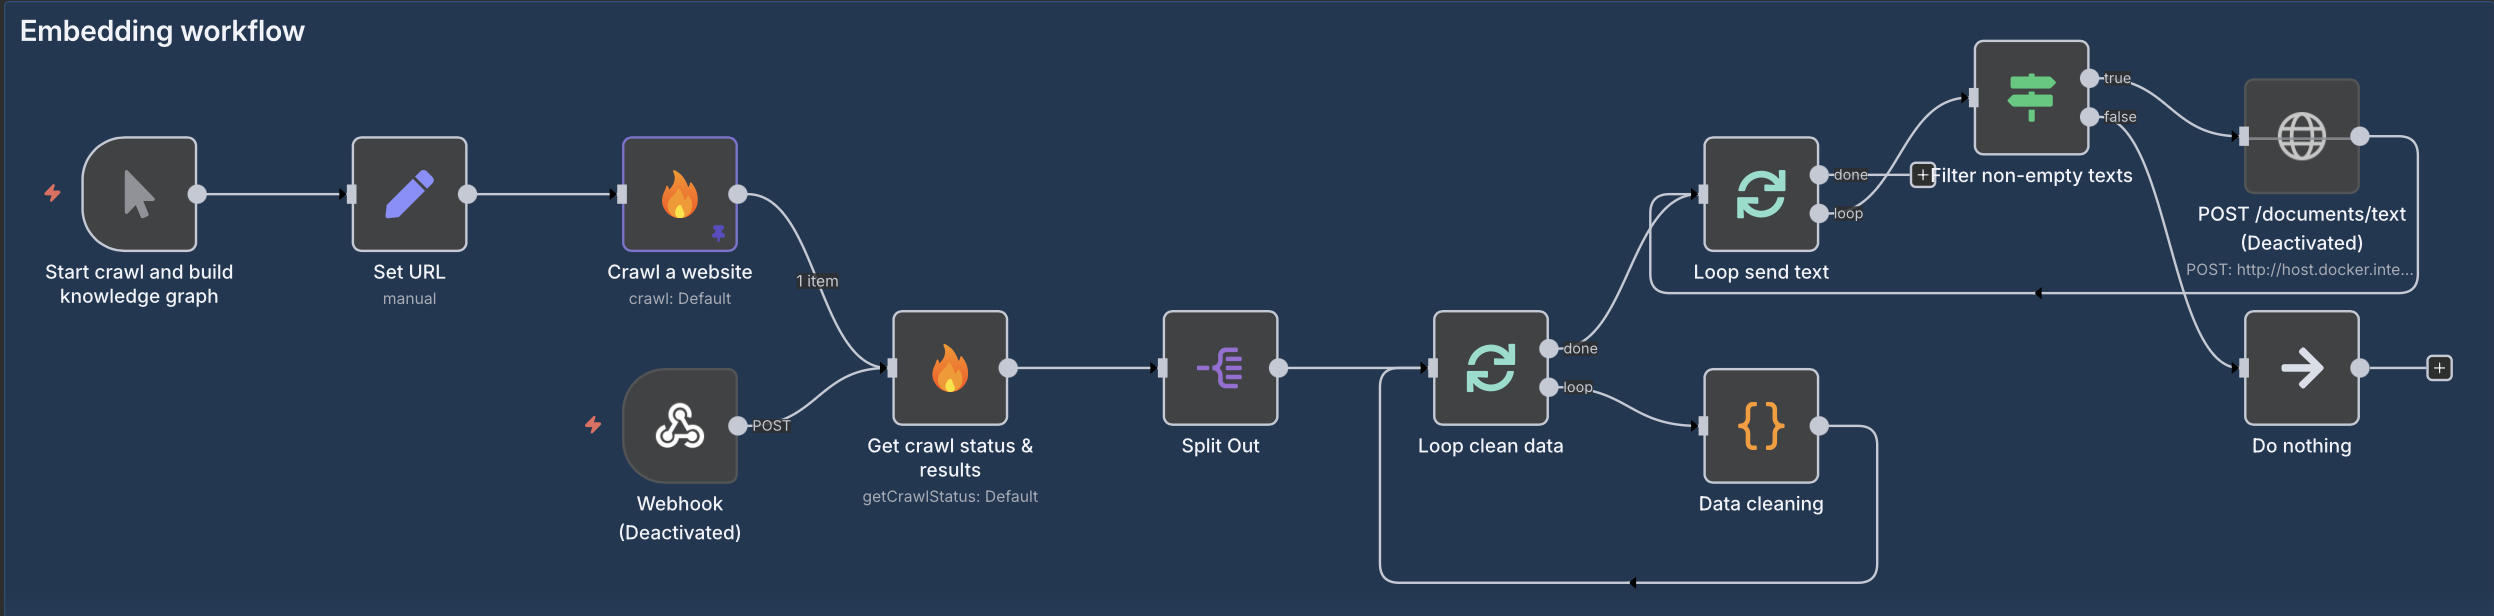
\includegraphics[width=\textwidth]{Figures/embed-new.png}
    \caption{Embedding pipeline: Firecrawl scrapes documentation, chunks are
        embedded via \texttt{bge-m3}, and entities/relations are extracted to
        build the knowledge graph.}
    \label{fig:rag_embed}
\end{figure}

\subsection{Knowledge Graph}

Figure~\ref{fig:rag_kg} shows the resulting knowledge graph for product
documentation. Nodes represent entities (features, concepts, actions), and
edges capture relationships. This structure enables retrieval to follow
semantic connections rather than relying solely on surface-level similarity.

\begin{figure}[htbp]
    \centering
    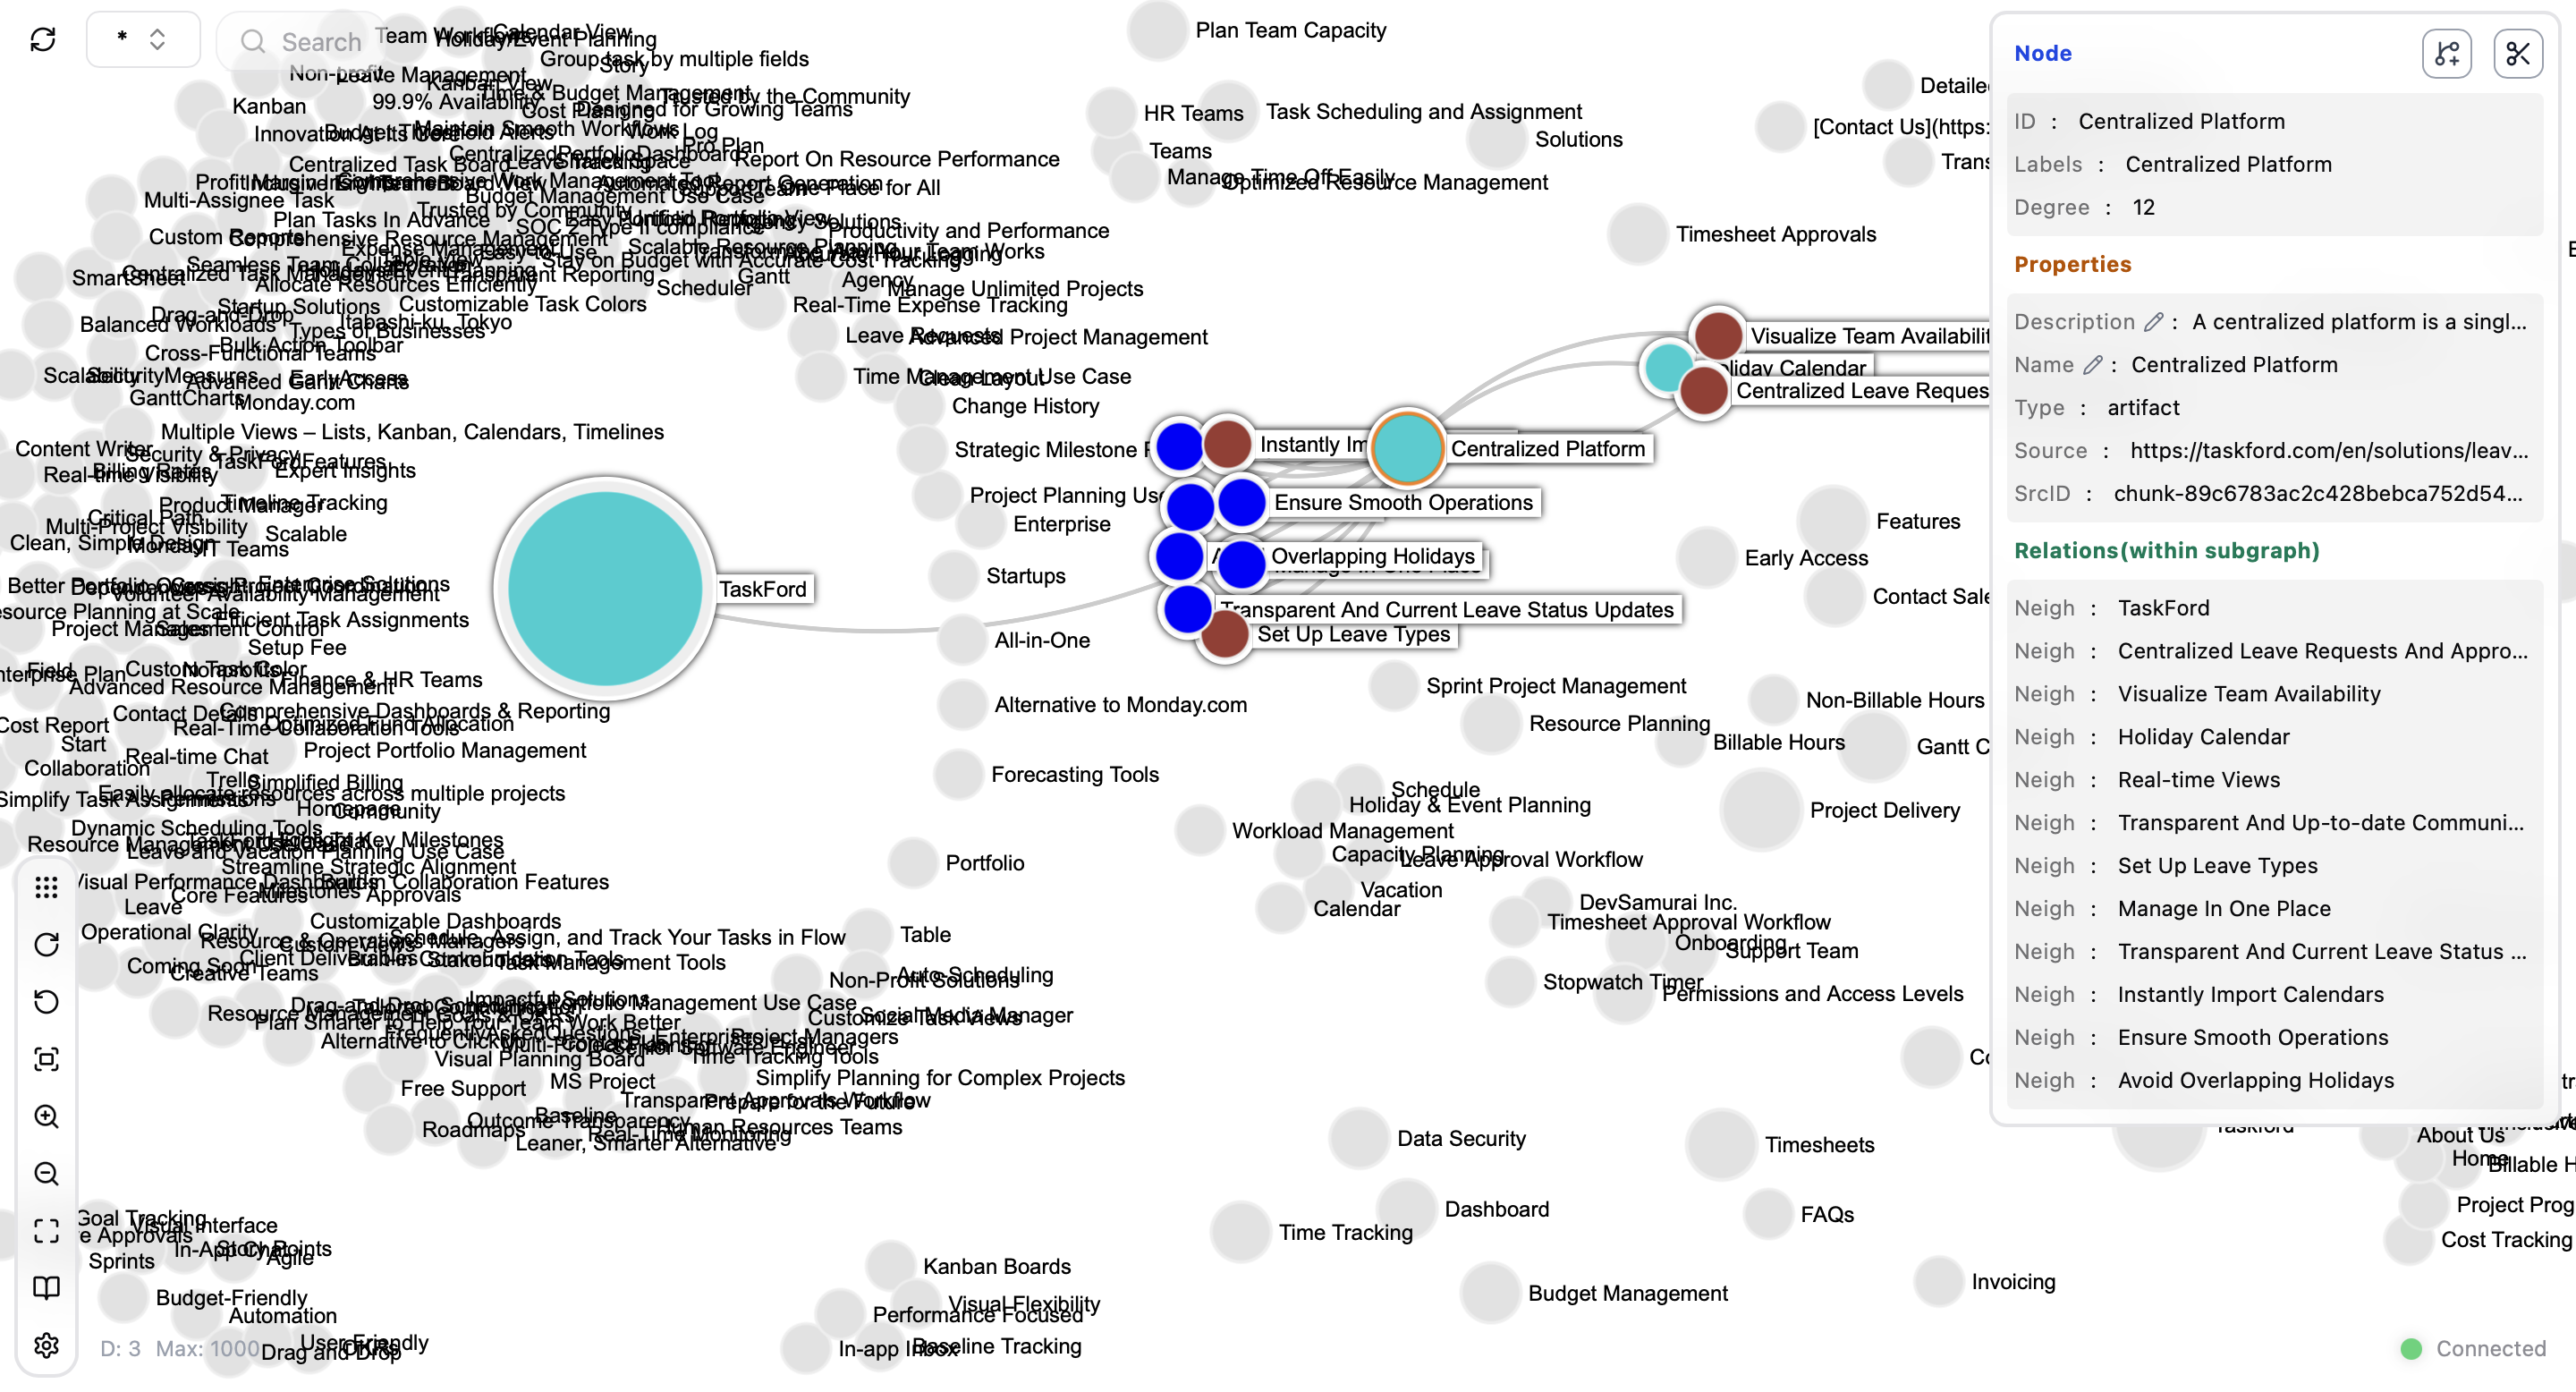
\includegraphics[width=0.9\textwidth]{Figures/knowledge-graph.png}
    \caption{Knowledge graph of product documentation showing entity nodes and
        relation edges. Graph-guided retrieval improves multi-hop query
        accuracy.}
    \label{fig:rag_kg}
\end{figure}

%=============================================================================
\section{Observations and Lessons}
\label{sec:RAG_Lessons}
%=============================================================================

Evaluation focused on grounding accuracy and response quality. LightRAG showed
clear improvements over naïve RAG:

\begin{itemize}
    \item Better faithfulness: answers aligned more closely with source
          documentation.
    \item Multi-hop capability: graph structure helped resolve queries
          requiring multiple conceptual hops.
    \item Anomaly detection: surfaced data quality issues (placeholder emails,
          incomplete content).
\end{itemize}

Challenges included verbose initial responses, addressed through prompt-level
constraints and answer-length controls. The hybrid retrieval approach added
latency compared to pure vector search but yielded meaningfully better
accuracy.

Key learning points:

\begin{itemize}
    \item Structure-aware retrieval (graph + vectors) materially improves RAG
          faithfulness over pure embeddings.
    \item Entity/relation extraction adds preprocessing cost but pays off in
          multi-hop scenarios.
    \item Data quality matters: RAG systems surface defects in source content;
          clean, well-structured documentation is critical.
    \item Answer verbosity requires explicit control; prompt engineering and
          output formatting are necessary for production readiness.
\end{itemize}

LightRAG demonstrated that thoughtful architectural choices in retrieval can
bridge the gap between naïve RAG and production-quality Q\&A systems.
